\documentclass[11pt,answers]{exam}
\usepackage[legalpaper,bindingoffset=0in,left=.6in,right=0.8in,top=0.4in,bottom=0.7in,headsep=.5\baselineskip]{geometry}
\usepackage[utf8]{inputenc}
\usepackage{graphicx}
\usepackage{listings}
\usepackage{enumitem}
\usepackage{amsmath}
\usepackage{multirow}
\usepackage{multicol}
\usepackage{caption}
\usepackage{tabularx}
\usepackage{url}
\usepackage{amssymb}
\usepackage{array}
\usepackage{tikz}
\usepackage{graphicx}
\usetikzlibrary{shapes.callouts, patterns, positioning, arrows.meta, shapes.geometric, shadows, calc, patterns, 3d, backgrounds, shadings}
\usepackage{adjustbox}
\usepackage{ragged2e}
\usepackage{pgfplots}

%\pagenumbering{gobble}
\def\changemargin#1#2{\list{}{\rightmargin#2\leftmargin#1}
\item[]}
\let\endchangemargin=\endlist
\usepackage{xcolor}
\usepackage{listings}
\definecolor{mGreen}{rgb}{0,0.6,0}
\definecolor{mGray}{rgb}{0.5,0.5,0.5}
\definecolor{mPurple}{rgb}{0.58,0,0.82}
\definecolor{backgroundColour}{rgb}{0.95,0.95,0.92}
\lstset{
  language=C,
  basicstyle=\ttfamily\small,
  aboveskip={1.0\baselineskip},
  belowskip={1.0\baselineskip},
  columns=fixed,
  extendedchars=true,
  breaklines=true,
  tabsize=4,
  prebreak=\raisebox{0ex}[0ex][0ex]{\ensuremath{\hookleftarrow}},
  frame=lines,
  showtabs=false,
  showspaces=false,
  showstringspaces=false,
  keywordstyle=\color[rgb]{0.627,0.126,0.941},
  commentstyle=\color[rgb]{0.133,0.545,0.133},
  stringstyle=\color[rgb]{01,0,0},
  numbers=left,
  numberstyle=\small,
  stepnumber=1,
  numbersep=10pt,
  captionpos=t,
escapeinside={\%*}{*)}
}
%\renewcommand\thequestion{Q.\arabic{question}}
%\renewcommand{\questionlabel}{\thequestion)}
%\renewcommand{\questionshook}{%
%\setlength{\leftmargin}{0pt}%
%\setlength{\labelwidth}{-\labelsep}%
%}

%\pointsinrightmargin
\pointsdroppedatright
%\marksnotpoints
%\marginpointname{ \points}
%\pointformat{\boldmath\themarginpoints}

\title{
\begin{changemargin}{0.68cm}{0.68cm}
  \normalsize Class Test 4\hfill {January 2025}\\
\end{changemargin}
\vspace{.4cm}
\large BANGLADESH UNIVERSITY OF ENGINEERING AND TECHNOLOGY\\
\vspace{.1cm}
Department of Computer Science and Engineering\\
\vspace{.2cm}
L-4/T-1 \hspace{.1cm} CSE 409: Computer Graphics\\
\vspace{.2cm}
\textbf{Time: 25 minutes} \hspace{2.2cm} \textbf{Marks: 20}
\begin{changemargin}{0.68cm}{0.68cm}
  \normalsize Student Name: \underline{Md. Ashrafur Rahman Khan} \hfill Student ID: \underline{1905005}\\
\end{changemargin}
}
\author{}
\date{}

\begin{document}

\maketitle
\thispagestyle{empty}
\begin{questions}
\vspace{-2cm}

\question[1]{
  What is the formula for the half-way vector in the Blinn-Phong model?
  \hfill (1)

  \begin{oneparchoices}
    \choice $\frac{\vec{L} + \vec{V}}{2}$
    \choice $\frac{\vec{L} + \vec{H}}{\sqrt{2}}$
    \choice $2(\vec{L}\cdot\vec{N})\vec{N} - \vec{L}$
    \choice  $\frac{\vec{L} + \vec{V}}{|\vec{L} + \vec{V}|}$ $\textcolor{green}{\checkmark}$
  \end{oneparchoices}
}

\question[1]{
  Ambient light is an approximation of | \hfill (1)

  \begin{oneparchoices}
    \choice Global illumination $\textcolor{green}{\checkmark}$
    \choice Path tracing
    \choice Shadows
    \choice Reflection
  \end{oneparchoices}
}

\question[1]{
  For the softest edges, we should use spot light falloff exponent $e = ?$
  \hfill (1)

  \begin{oneparchoices}
    \choice 0
    \choice 2
    \choice 10
    \choice 20 $\textcolor{green}{\checkmark}$
  \end{oneparchoices}
}

\question[1]{
  Which type of camera preserves distances? \hfill (1)

  \begin{oneparchoices}
    \choice Pinhole
    \choice Simple field
    \choice Fisheye
    \choice Orthographic $\textcolor{green}{\checkmark}$
  \end{oneparchoices}
}

\question[1]{
  Which is not a feature of the simplified pinhole camera? \hfill (1)

  \begin{oneparchoices}
    \choice Non-inverted image
    \choice Perspective distortion $\textcolor{green}{\checkmark}$
    \choice Depth of field effect $\textcolor{green}{\checkmark}$
    \choice Unrealizable
  \end{oneparchoices}
}

\question[]
{
  \begin{multicols}{2}
    Same triangle again! But now we want to texture it with an image.
    The $(u, v)$ coordinates of the vertices $A$, $B$ and $C$ are $(0, 0)$, $(1, 0)$ and $(0.5, 1)$ respectively.

    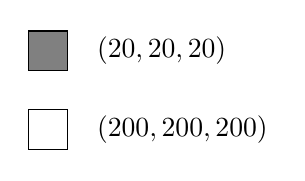
\begin{tikzpicture}
      \draw[black,fill=gray] (0,0) rectangle (0.5,0.5);
      \node[right] at (0.75, 0.25) {$(20,20,20)$};
      \draw[black,fill=white] (0,-1) rectangle ++(0.5,0.5);
      \node[right] at (0.75, -0.75) {$(200,200,200)$};
    \end{tikzpicture}

    \vfill
    \columnbreak
    \centering
    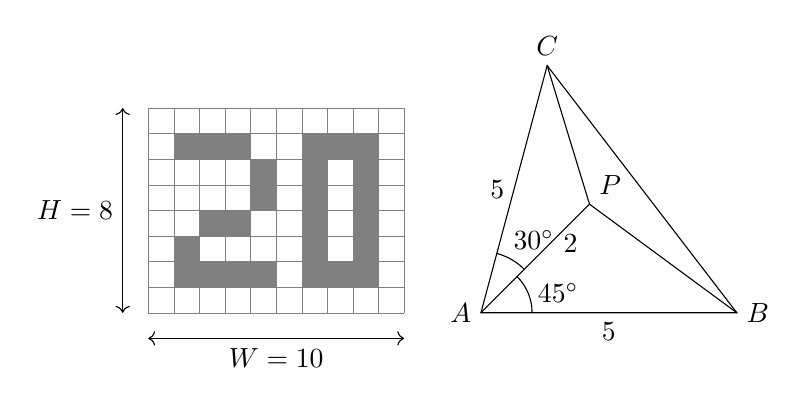
\begin{tikzpicture}[scale=0.65]
      \draw[step=0.5cm, gray, very thin] (0,0) grid (5,4);  \tikzstyle{pixel} = [fill=gray]

      \foreach \x/\y in {
        0.5/3, 1/3, 1.5/3,
        2/2.5, 2/2,
        1/1.5,1.5/1.5,0.5/1,
        0.5/0.5, 1/0.5, 1.5/0.5, 2/0.5
      } {
        \fill[pixel] (\x,\y) rectangle ++(0.5,0.5);
      }

      \foreach \x/\y in {
        3/3, 3.5/3, 4/3,
        3/2.5, 4/2.5,
        3/2, 4/2,
        3/1.5, 4/1.5,
        3/1, 4/1,
        3/0.5, 3.5/0.5, 4/0.5
      } {
        \fill[pixel] (\x,\y) rectangle ++(0.5,0.5);
      }
      \draw[<->] (0, -0.5) -- (5, -0.5) node[midway, below] {$W=10$};
      \draw[<->] (-0.5, 0) -- (-0.5, 4) node[midway, left] {$H=8$};

      \begin{scope}[xshift=6.5cm]
        \coordinate (A) at (0, 0);
        \coordinate (B) at (0:5);
        \coordinate (C) at (75:5);
        \coordinate (P) at (45:3);
        \draw (A) node[left] {$A$}  -- node[midway,below] {$5$} (B) node[right] {$B$} -- (C) node[above] {$C$} -- node[midway,left] {$5$} cycle;
        \draw (A) -- (P) node[midway, above, shift={(0.45,-0.05)}] {$2$};
        \draw (B) -- (P) node[above right] {$P$};
        \draw (C) -- (P);
        \draw (1,0) arc [start angle=0, end angle=45, radius=1cm]
        node[midway, right] {$45^{\circ}$};
        \draw (45:1.2) arc [start angle=45, end angle=75, radius=1.2cm]
        node[midway, above right,xshift=-0.1cm] {$30^{\circ}$};
      \end{scope}
    \end{tikzpicture}

  \end{multicols}

a) What is the colour of $P$ using nearest neighbour interpolation?  \hfill (3) \\

\textbf{Answer:} From CT-3 we get :3,
\begin{align*}
  \alpha = 0.5, \quad
  \beta = 0.207, \quad
  \gamma = 0.293
\end{align*}

Therefore, the $(u, v)$ coordinates of $P$ are,
\begin{align*}
  u = \alpha \cdot 0 + \beta \cdot 1 + \gamma \cdot 0.5 = 0.3535 \\
  v = \alpha \cdot 0 + \beta \cdot 0 + \gamma \cdot 1 = 0.293
\end{align*}

We also have, $w = W - 1 = 9$ and $h = H - 1 = 7$.
\begin{align*}
  \text{color}(P) &= T\left[ \operatorname{round}(u \cdot w), \operatorname{round}(v \cdot h) \right] \\
  &= T\left[ \operatorname{round}(0.3535 \cdot 9), \operatorname{round}(0.293 \cdot 7) \right] \\
  &= T[3, 2] = \text{rgb}(200, 200, 200)
\end{align*}

b) What is the colour of $P$ using bilinear interpolation?  \hfill (3)
{
\footnotesize
\begin{multicols}{2}
  We can see that the corner colours are:
  \begin{align*}
    c_{00} &= T\left[ \lfloor u \cdot w \rfloor, \lfloor v \cdot h \rfloor \right] = T[3, 2] = \text{rgb}(200, 200, 200) \\
    c_{10} &= T\left[ \lfloor u \cdot w \rfloor + 1, \lfloor v \cdot h \rfloor \right] = T[4, 2] = \text{rgb}(200, 200, 200) \\
    c_{01} &= T\left[ \lfloor u \cdot w \rfloor, \lfloor v \cdot h \rfloor + 1 \right] = T[3, 3] = \text{rgb}(20, 20, 20) \\
    c_{11} &= T\left[ \lfloor u \cdot w \rfloor + 1, \lfloor v \cdot h \rfloor + 1 \right] = T[4, 3] = \text{rgb}(200, 200, 200) \\
  \end{align*}

  Now, we can calculate the interpolation factors:
  \begin{align*}
    t_u &= u \cdot w - \lfloor u \cdot w \rfloor = 0.3535 \cdot 9 - 3 = 0.1805 \\
    t_v &= v \cdot h - \lfloor v \cdot h \rfloor = 0.293 \cdot 7 - 2 = 0.051 \\
  \end{align*}

  Therefore, the final colour is,
  \begin{align*}
    \text{color}(P) &= \text{lerp}(\text{lerp}(c_{00}, c_{10}, t_u), \text{lerp}(c_{01}, c_{11}, t_u), t_v) \\
    &= \text{lerp}(\text{rgb}(200, 200, 200), \\
    & \quad \quad \text{lerp}(\text{rgb}(20, 20, 20), \text{rgb}(200, 200, 200), 0.1805), 0.051) \\
    &= \text{lerp}(\text{rgb}(200, 200, 200), \text{rgb}(52.49,52.49,52.49), 0.051) \\
    &\approx \text{rgb}(192.477, 192.477, 192.477) \\
    &= \text{rgb}(192, 192, 192)
  \end{align*}

\end{multicols}
}
}
\newpage
\question[]
{
\begin{multicols}{2}

As a game developer in Iron studio, you are working in a new level of a game.
There is just a strange ball at $(10,5,0)$ of radius 5 and a point light at $(2,11,0)$.\\
After much thought, you have decided the following parameters using the Phong model:
\begin{itemize}
  \item Point light intensity $\mathbf{I} = (20, 20, 20)$
  \item Ambient light $\mathbf{I}_a = (0.1, 0.1, 0.1)$
  \item Ambient Coefficient $\mathbf{k}_a = (0.1, 0.1, 0.1)$
  \item Diffuse Coefficient $\mathbf{k}_d = (0.4, 0.4, 0.4)$
  \item Specular Coefficient $\mathbf{k}_s = (0.5, 0.5, 0.5)$
  \item Shininess $n = 10$
\end{itemize}
\vfill
\columnbreak
\begin{center}
  \footnotesize
  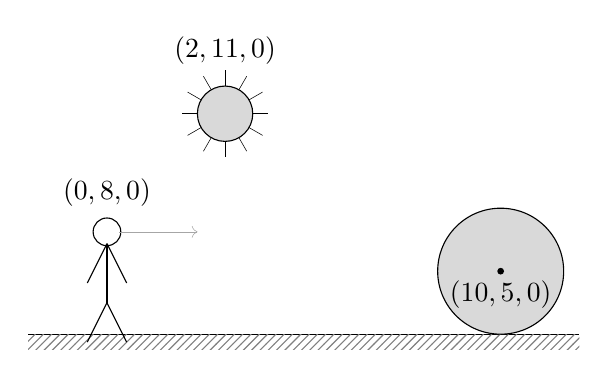
\begin{tikzpicture}
    \draw[black] (-6,-0.8) -- (1,-0.8);
    \fill[pattern=north east lines, pattern color=gray] (-6,-0.8) rectangle (1,-1);
    \draw[black,fill=gray!30] (0,0) circle (0.8cm);
    \draw[black,fill=black] (0,0) circle (1pt) node[below] {$(10,5,0)$};

    % stick man
    \draw[black] (-5,0.35) --++(0,-0.75);
    \draw[black] (-5,0.35) --++(-0.25,-0.5);
    \draw[black] (-5,0.35) --++(0.25,-0.5);
    \draw[black] (-5,-0.4) --++(-0.25,-0.5);
    \draw[black] (-5,-0.4) --++(0.25,-0.5);
    \draw[black] (-5,0.5) circle (5pt);

    \draw[gray!70,very thin,->] (-4.85,0.5) --++(1,0);
    \node[above] at (-5,0.7) {$(0,8,0)$};

    \begin{scope}[shift={(-3.5,2)}]
      \foreach \t in {0, 30, ..., 360} {
        \draw[very thin] (0,0) -- (\t:0.55);
      }
      \draw[black,fill=gray!30] (0,0) circle (10pt);
      \node[above] at (0,0.5) {$(2,11,0)$};
    \end{scope}

  \end{tikzpicture}

\end{center}
\end{multicols}

But your game designer says the
scene doesn't look right. She says the ball should be bluish gray in shadow [rgb(0,10,20)].
She also says the material should be less shiny. When the character at $(0,8,0)$ looks straight
ahead (in the direction of x), he should see a gray colour [rgb(115,125,135)].

(\textbf{Hint:} Normalize RGB colours to $(0, 1)$ range.)

a) As per your game designer's requirement, what should be the value of the ambient coefficient $\mathbf{k}_a$? \hfill (3) \\

\textbf{Answer:} When the ball is in shadow, only ambient light contributes to the colour. Therefore,
\begin{align*}
\text{colour}_{\text{shadow}} &= \mathbf{I}_a \odot \mathbf{k}_a \\
\left(0, \frac{10}{255}, \frac{20}{255}\right) &= (0.1, 0.1, 0.1) \odot \mathbf{k}_a \\
\mathbf{k}_a = \left(0, \frac{10}{25.5}, \frac{20}{25.5}\right) &= (0, 0.392, 0.784)
\end{align*}

b) What should be the value of shininess $n$? \hfill (3) \\
}

\textbf{Answer:}
\begin{center}

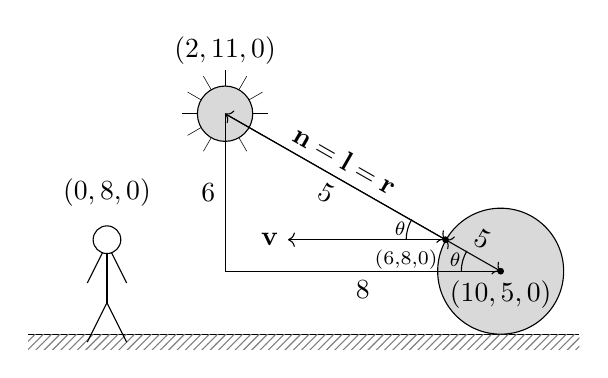
\begin{tikzpicture}
\draw[black] (-6,-0.8) -- (1,-0.8);
\fill[pattern=north east lines, pattern color=gray] (-6,-0.8) rectangle (1,-1);
\draw[black,fill=gray!30] (0,0) circle (0.8cm);
\draw[black,fill=black] (0,0) circle (1pt) node[below] {$(10,5,0)$};

% stick man
\draw[black] (-5,0.35) --++(0,-0.75);
\draw[black] (-5,0.35) --++(-0.25,-0.5);
\draw[black] (-5,0.35) --++(0.25,-0.5);
\draw[black] (-5,-0.4) --++(-0.25,-0.5);
\draw[black] (-5,-0.4) --++(0.25,-0.5);
\draw[black,fill=white] (-5,0.4) circle (5pt);

\draw[black, ->] (-0.7,0.4) --++ (-2, 0) node[left] {$\mathbf{v}$};
\node[above] at (-5,0.7) {$(0,8,0)$};

\begin{scope}[shift={(-3.5,2)}]
\foreach \t in {0, 30, ..., 360} {
\draw[very thin] (0,0) -- (\t:0.55);
}
\draw[black,fill=gray!30] (0,0) circle (10pt);
\node[above] at (0,0.5) {$(2,11,0)$};
\end{scope}

\draw[black,fill=black] (-0.7,0.4) circle (1pt) node[above, shift={(-0.5,-0.5)}] {\scriptsize (6,8,0)};
\draw[-] (-3.5,2) -- (-0.7,0.4) node[midway, above, sloped] {{$\mathbf{n} = \mathbf{l} = \mathbf{r}$}};
\draw[<->] (-3.5,2) -- (-0.7,0.4) node[midway, below, sloped] {$5$};
\draw[<->] (0,0) -- (-0.7,0.4) node[midway, above, sloped] {$5$};
\draw[-] (-3.5,0) -- (0, 0) node[midway, below, sloped] {$8$};
\draw[-] (-3.5,2) -- (-3.5, 0) node[midway, left] {$6$};

\draw (-0.5, 0) arc [start angle=180, end angle=149, radius=0.5cm] node[midway, above left,shift={(0.1, -0.2)}] {\scriptsize $\theta$};
\draw (-1.2, 0.4) arc [start angle=180, end angle=149, radius=0.5cm] node[midway, above left,shift={(0.1, -0.2)}] {\scriptsize $\theta$};
\end{tikzpicture}
\end{center}

Now, to calculate the final colour, we need to know the angles or rather the dot products $\mathbf{n} \cdot \mathbf{l}$ and $\mathbf{r} \cdot \mathbf{v}$.
Since the surface is a sphere, the normal points in the direction of the light. The light is also reflected in the same direction as the normal.
So, $\mathbf{n} = \mathbf{l} = \mathbf{r}$ and $\mathbf{n} \cdot \mathbf{l} = 1$.

The angle between $\mathbf{v}$ and $\mathbf{n}$ is the angle $\theta$ which is the angle between the sides 10 and 8, in the right triangle with sides 6, 8 and 10 between
the light and the sphere center. Therefore,
\begin{align*}
\mathbf{v} \cdot \mathbf{n} = \mathbf{v} \cdot \mathbf{r} = \cos \theta = \frac{8}{10} = 0.8
\end{align*}

Also, we need to consider the light attenuation due to distance. The distance between the light and the point on the sphere is 5.

So, now th final colour is,
\begin{align*}
\text{colour} &= \mathbf{I}_a \odot \mathbf{k}_a + \frac{1}{d^2} \left[ \mathbf{I} \odot \mathbf{k}_d (\mathbf{n} \cdot \mathbf{l}) + \mathbf{I} \odot \mathbf{k}_s (\mathbf{r} \cdot \mathbf{v})^n \right] \\
\left(\frac{115}{255},\frac{125}{255},\frac{135}{255}\right) &= \left(\frac{0}{255},\frac{10}{255},\frac{20}{255}\right) + \frac{1}{5^2} \left[ (20, 20, 20) \odot (0.4, 0.4, 0.4) (1) + (20, 20, 20) \odot (0.5, 0.5, 0.5) (0.8)^n \right] \\
\end{align*}
Solving for the $n$ in the R component, we get,
\begin{align*}
\frac{115}{255} &= 0 + \frac{1}{25} \left[ 8 + 10 (0.8)^n \right] \\
(0.8)^n &= \frac{\frac{115 \cdot 25}{255} - 8 }{ 10} = \frac{167}{510} \\
n &= \log_{0.8} \frac{167}{510}\approx 5.003 \approx 5
\end{align*}

\question[]For your hard work and attending the exam so early in the morning.\hfill (3) \\
\textbf{Answer:} Thanks, I suppose.
\end{questions}
\end{document}